\documentclass[border={1.5mm 0.6mm}]{standalone}
\usepackage[T1]{fontenc}
\usepackage{newtxtext,newtxmath}
\usepackage{xcolor}
\usepackage{tikz}
\usepackage{pgfplots}
\usepackage{amsmath}
\pgfplotsset{compat=1.18}
\usetikzlibrary{arrows.meta,calc,positioning,decorations.pathreplacing,fit,backgrounds,patterns,shapes.misc,shapes.geometric}
\usepgfplotslibrary{groupplots,fillbetween}
\definecolor{ink}{HTML}{111111}
\definecolor{accent}{HTML}{A8321F}
\definecolor{steel}{HTML}{1F4A7A}
\definecolor{midgray}{HTML}{6E6E6E}
\definecolor{lightgray}{HTML}{D9D9D9}
\newcommand{\figsize}{\fontsize{8}{9.6}\selectfont}
\newcommand{\smallsize}{\fontsize{7}{8.4}\selectfont}
\AtBeginDocument{\DeclareFontShape{OML}{ntxmi}{m}{it}{<-> ntxmi}{}\frenchspacing}
\pgfplotsset{
  every axis/.append style={
    axis line style={line width=0.45pt,ink},
    tick style={line width=0.4pt,ink},
    major tick length=3pt,
    minor tick length=1.6pt,
    tick align=inside,
    xtick pos=both,
    ytick pos=both,
    minor tick num=0,
    grid=none,
    label style={font=\figsize},
    tick label style={font=\figsize},
    legend style={font=\smallsize,draw=none,fill=none,inner sep=1pt,row sep=-0.5pt},
    legend cell align=left,
    xlabel near ticks,
    ylabel near ticks,
    /pgf/number format/1000 sep={\mbox{,}},
    scaled ticks=false,
    clip marker paths=true,
  },
  x25519/.style={ink,line width=0.5pt,solid,mark=*,mark size=1.0pt,mark options={solid,fill=ink,line width=0.2pt}},
  hybrid/.style={accent,line width=0.5pt,solid,mark=square*,mark size=0.95pt,mark options={solid,fill=accent,line width=0.2pt}},
  x25519open/.style={ink,only marks,mark=*,mark size=1.25pt,mark options={solid,fill=white,line width=0.45pt}},
  hybridopen/.style={accent,only marks,mark=square*,mark size=1.15pt,mark options={solid,fill=white,line width=0.45pt}},
}
\newcommand{\panel}[1]{{\figsize(#1)}}

\tikzset{
  rail/.style={line width=0.55pt,ink},
  msg/.style={line width=0.45pt,ink,-{Latex[length=2.6pt,width=1.7pt]}},
  msgplain/.style={line width=0.45pt,ink},
  lostmsg/.style={line width=0.45pt,ink,dash pattern=on 1.6pt off 1.1pt},
  paritymsg/.style={line width=0.55pt,steel,-{Latex[length=2.6pt,width=1.7pt]}},
  cross/.style={line width=0.6pt,ink},
  rebuilt/.style={line width=0.5pt,steel,fill=white},
  donetick/.style={line width=0.9pt,ink},
  brc/.style={decorate,decoration={brace,amplitude=2.6pt},line width=0.4pt,ink},
  gridline/.style={line width=0.3pt,lightgray},
  axisline/.style={line width=0.45pt,ink},
  lab/.style={font=\figsize,inner sep=0pt},
  sml/.style={font=\smallsize,inner sep=0pt},
}
\begin{document}
\figsize
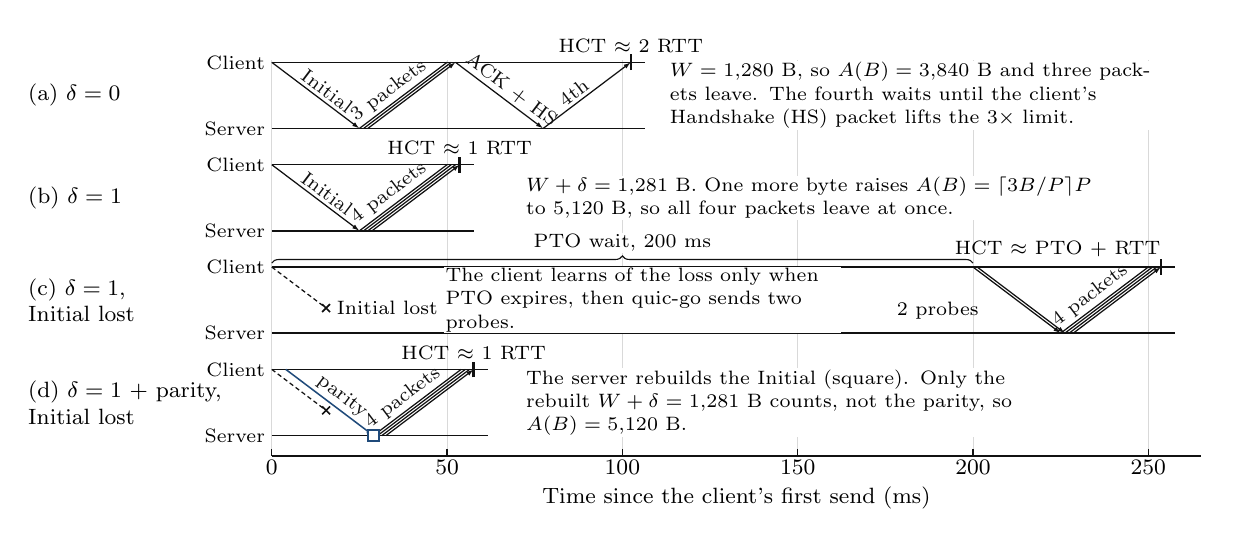
\begin{tikzpicture}[x=1mm,y=1mm]
\path (0,0) rectangle (150,62.40);
\draw[gridline] (31.000,8.000) -- (31.000,58.300);
\draw[gridline] (53.264,8.000) -- (53.264,58.300);
\draw[gridline] (75.528,8.000) -- (75.528,58.300);
\draw[gridline] (97.792,8.000) -- (97.792,58.300);
\draw[gridline] (120.057,8.000) -- (120.057,58.300);
\draw[gridline] (142.321,8.000) -- (142.321,58.300);
\node[lab,anchor=west,align=left] at (0,53.800) {(a) $\delta=0$};
\draw[rail] (31.000,58.000) -- (78.378,58.000);
\draw[rail] (31.000,49.600) -- (78.378,49.600);
\node[sml,anchor=east] at (30.200,58.000) {Client};
\node[sml,anchor=east] at (30.200,49.600) {Server};
\draw[msg] (31.000,58.000) -- node[sml,text=ink,sloped,pos=0.56,above=0.2mm,inner sep=0.2mm] {Initial} (42.132,49.600);
\draw[msgplain] (42.132,49.600) -- node[sml,text=ink,sloped,pos=0.42,above=0.2mm,inner sep=0.2mm] {3 packets} (53.264,58.000);
\draw[msgplain] (42.666,49.600) -- (53.798,58.000);
\draw[msg] (43.201,49.600) -- (54.333,58.000);
\draw[msg] (54.333,58.000) -- node[sml,text=ink,sloped,pos=0.56,above=0.2mm,inner sep=0.2mm] {ACK + HS} (65.465,49.600);
\draw[msg] (65.465,49.600) -- node[sml,text=ink,sloped,pos=0.42,above=0.2mm,inner sep=0.2mm] {4th} (76.597,58.000);
\draw[donetick] (76.597,57.000) -- (76.597,59.000);
\node[sml,anchor=south] at (76.597,59.200) {HCT $\approx$ 2 RTT};
\node[sml,anchor=west,align=left,text width=62.0mm,fill=white,inner sep=0.5pt] at (81.317,53.800) {\hyphenpenalty=10000\exhyphenpenalty=10000 ${W=1{,}280}$~B, so ${A(B)=3{,}840}$~B and three packets leave. The fourth waits until the client's Handshake (HS) packet lifts the 3$\times$ limit.};
\node[lab,anchor=west,align=left] at (0,40.800) {(b) $\delta=1$};
\draw[msgplain] (42.132,36.600) -- node[sml,text=ink,sloped,pos=0.42,above=0.2mm,inner sep=0.2mm] {4 packets} (53.264,45.000);
\draw[msgplain] (42.666,36.600) -- (53.798,45.000);
\draw[msgplain] (43.201,36.600) -- (54.333,45.000);
\draw[msg] (43.735,36.600) -- (54.867,45.000);
\draw[rail] (31.000,45.000) -- (56.648,45.000);
\draw[rail] (31.000,36.600) -- (56.648,36.600);
\node[sml,anchor=east] at (30.200,45.000) {Client};
\node[sml,anchor=east] at (30.200,36.600) {Server};
\draw[msg] (31.000,45.000) -- node[sml,text=ink,sloped,pos=0.56,above=0.2mm,inner sep=0.2mm] {Initial} (42.132,36.600);
\draw[donetick] (54.867,44.000) -- (54.867,46.000);
\node[sml,anchor=south] at (54.867,46.200) {HCT $\approx$ 1 RTT};
\node[sml,anchor=west,align=left,text width=72.0mm,fill=white,inner sep=0.5pt] at (63.060,40.800) {\hyphenpenalty=10000\exhyphenpenalty=10000 ${W+\delta=1{,}281}$~B. One more byte raises ${A(B)=\lceil 3B/P\rceil P}$ to $5{,}120$~B, so all four packets leave at once.};
\node[lab,anchor=west,align=left] at (0,27.800) {(c) $\delta=1$,\\Initial lost};
\draw[rail] (31.000,32.000) -- (145.705,32.000);
\draw[rail] (31.000,23.600) -- (145.705,23.600);
\node[sml,anchor=east] at (30.200,32.000) {Client};
\node[sml,anchor=east] at (30.200,23.600) {Server};
\draw[lostmsg] (31.000,32.000) -- (37.902,26.792);
\draw[cross] (37.402,26.292) -- (38.402,27.292) (37.402,27.292) -- (38.402,26.292);
\node[sml,anchor=west,inner sep=0.3pt] at (39.102,26.792) {Initial lost};
\draw[msg] (120.057,32.000) -- (131.189,23.600);
\draw[msg] (120.591,32.000) -- (131.723,23.600);
\node[sml,anchor=east,align=right,inner sep=0.3pt] at (120.947,26.400) {2 probes};
\draw[msgplain] (131.189,23.600) -- node[sml,text=ink,sloped,pos=0.42,above=0.2mm,inner sep=0.2mm] {4 packets} (142.321,32.000);
\draw[msgplain] (131.723,23.600) -- (142.855,32.000);
\draw[msgplain] (132.257,23.600) -- (143.389,32.000);
\draw[msg] (132.792,23.600) -- (143.924,32.000);
\draw[brc] (31.000,32.500) -- (120.057,32.500);
\node[sml,anchor=south,fill=white,inner sep=0.4pt] at (75.528,33.750) {PTO wait, 200 ms};
\draw[donetick] (143.924,31.000) -- (143.924,33.000);
\node[sml,anchor=south east] at (143.924,33.200) {HCT $\approx$ PTO + RTT};
\node[sml,anchor=west,align=left,text width=50.0mm,fill=white,inner sep=0.5pt] at (52.819,27.800) {\hyphenpenalty=10000\exhyphenpenalty=10000 The client learns of the loss only when PTO \mbox{expires}, then quic-go sends two probes.};
\node[lab,anchor=west,align=left] at (0,14.800) {(d) $\delta=1$ + parity,\\Initial lost};
\draw[msgplain] (43.913,10.600) -- node[sml,text=ink,sloped,pos=0.42,above=0.2mm,inner sep=0.2mm] {4 packets} (55.045,19.000);
\draw[msgplain] (44.448,10.600) -- (55.580,19.000);
\draw[msgplain] (44.982,10.600) -- (56.114,19.000);
\draw[msg] (45.516,10.600) -- (56.648,19.000);
\draw[rail] (31.000,19.000) -- (58.429,19.000);
\draw[rail] (31.000,10.600) -- (58.429,10.600);
\node[sml,anchor=east] at (30.200,19.000) {Client};
\node[sml,anchor=east] at (30.200,10.600) {Server};
\draw[lostmsg] (31.000,19.000) -- (37.902,13.792);
\draw[cross] (37.402,13.292) -- (38.402,14.292) (37.402,14.292) -- (38.402,13.292);
\draw[paritymsg] (32.781,19.000) -- node[sml,text=ink,sloped,pos=0.56,above=0.2mm,inner sep=0.2mm] {parity} (43.913,10.600);
\draw[rebuilt] (43.213,9.900) rectangle (44.613,11.300);
\draw[donetick] (56.648,18.000) -- (56.648,20.000);
\node[sml,anchor=south] at (56.648,20.200) {HCT $\approx$ 1 RTT};
\node[sml,anchor=west,align=left,text width=72.0mm,fill=white,inner sep=0.5pt] at (63.060,14.800) {\hyphenpenalty=10000\exhyphenpenalty=10000 The server rebuilds the Initial (square). Only the rebuilt ${W+\delta=1{,}281}$~B counts, not the parity, so ${A(B)=5{,}120}$~B.};
\draw[axisline] (31.000,8.000) -- (31.000,8.900);
\node[lab,anchor=north] at (31.000,7.500) {0};
\draw[axisline] (53.264,8.000) -- (53.264,8.900);
\node[lab,anchor=north] at (53.264,7.500) {50};
\draw[axisline] (75.528,8.000) -- (75.528,8.900);
\node[lab,anchor=north] at (75.528,7.500) {100};
\draw[axisline] (97.792,8.000) -- (97.792,8.900);
\node[lab,anchor=north] at (97.792,7.500) {150};
\draw[axisline] (120.057,8.000) -- (120.057,8.900);
\node[lab,anchor=north] at (120.057,7.500) {200};
\draw[axisline] (142.321,8.000) -- (142.321,8.900);
\node[lab,anchor=north] at (142.321,7.500) {250};
\draw[axisline] (31.000,8.000) -- (149.000,8.000);
\node[lab,anchor=north] at (90.000,4.100) {Time since the client's first send (ms)};
\pgfresetboundingbox
\path (0,0) rectangle (150,62.40);
\end{tikzpicture}
\end{document}
